\documentclass[aps,prl,twocolumn,showpacs,amsmath,amssymb]{revtex4-1}
%\documentclass[aps,prl,twocolumn,showpacs,preprintnumbers,amsmath,amssymb,citeautoscript]{revtex4-1}
%\documentclass[prl,showpacs,amssymb,amsmath,twocolumn]{revtex4-1}
%%%%%%%%%%%%
\usepackage{bookmath} % definitions and shortcuts
%%%%%%%%%%%%
\usepackage{graphicx}
\usepackage{amsmath}
\usepackage{color}
\newcommand{\blue}{\textcolor{blue}}
\newcommand{\red}{\textcolor{red}}
\newcommand{\cecoin}{CeCoIn$_5$} 
\def\opp#1{{\overline{ #1}}}


\bibliographystyle{apsrev4-1}
%~~~~~~~~~~~~~~~~~~~~~~~~~~~~~~~~~~~~~~~~~~~~~~~~~~~~~~~~~~~~~~~~~~~~~~~~~~~~~~~%
\begin{document}
%~~~~~~~~~~~~~~~~~~~~~~~~~~~~~~~~~~~~~~~~~~~~~~~~~~~~~~~~~~~~~~~~~~~~~~~~~~~~~~~%
\title{Electronic Spin Susceptibility Enhancement in Pauli Limited Unconventional Superconductors}

\author{Benjamin~M.~Rosemeyer}
\author{Anton~B.~Vorontsov}

\affiliation{Department of Physics, Montana State University, Montana 59717, USA}

\date{\today}

\begin{abstract}
%
We calculate the wave-vector dependent electronic spin susceptibility 
$\chi_{\alpha\beta}(\vq, \vH_0)$ 
of a superconducting state in uniform magnetic field $\vH_0$. 
We consider Pauli-limited superconductivity with $d$-wave symmetry, and a 2D cylindrical 
Fermi surface.  
We find that both longitudinal and transverse components of the susceptibility tensor are enhanced over their
normal state values, 
and we identify several wave vectors $\{\vq_\perp,\vq_\parallel\}$, 
that correspond to the maxima of either $\chi_\perp$ or $\chi_\parallel$. 
We compare our results with data on the high-field phase in heavy-fermion \cecoin. 
%
\end{abstract} 

\pacs{74.20.Rp,74.25.Ha,74.70.Tx} 

%74.20.Rp 	Pairing symmetries (other than s-wave) 
%74.25.Ha	Magnetic properties including vortex structures and related phenomena 
%74.25.Dw 	Superconductivity phase diagrams 
%74.70.Tx	Heavy-fermion superconductors

\maketitle


%~~~~~~~~~~~~~~~~~~~~~~~~~~~~~~~~~~~~~
%\emph{Introduction.}
%~~~~~~~~~~~~~~~~~~~~~~~~~~~~~~~~~~~~~
%
The interplay of superconductivity and magnetism, connected by the spin degree of freedom, 
for many years has been an active topic of research.
Singlet superconductivity with spin-zero pairs is competing with ferromagnetic order whose 
fields vary on length scales comparable to the size of Cooper pairs $\xi_0$.
This competition usually results in suppression of one of the orders. \cite{bulaevskii85}
%, but sometimes leads to more exotic states such as non-uniform Fulde-Ferrell-Larkin-Ovchinnikov (FFLO) 
%state.\cite{bulaevskii85,ful64,*lar64}
The antiferromagnetic order, on the other hand, with atomic-scale field oscillations, 
interferes much less with superconductivity.\cite{anderson_suhl59} 
Moreover, in unconventional superconductors the aniferromagnetic spin-density wave (SDW) order 
and superconducting condensate are attractive under certain conditions.\cite{machida87_sdw_hf,*kato87_sdw_hf}

Recent years have seen another cycle of interest in understanding the details of the SC-SDW interactions 
due to discovery of 
iron-based superconductors\cite{Johnston2010_review} 
and 
Ce-family of heavy-fermion materials\cite{Petrovic01_ce115,  Kenzelmann08_Qphase}.
In pnictides the co-existence of the SDW and SC is due to the multi-band nature 
and unconventional order parameter structure, and the interplay of two orders is a  
strong function of the 
Fermi surface topology.\cite{vor10_sc_sdw,*Fernandes2010_sdw_sc}
In heavy-fermion Pauli-limited \cecoin\ the normal state is non-magnetic but the SDW magnetism 
appears in the high-field low-temperature part of the diagram, through a second order transition, 
and diasapperas once the superconducting order disappears at first-order $H_{c2}$ transition. 
\cite{Bianchi2003_fflo, Kenzelmann08_Qphase, Kenzelmann10_Qphase}
The experiments point towards strong AFM fluctuations in the normal state,\cite{Paglione03_qcp115,*Bianchi03_qcp115} 
which, however, are not 
strong enough to produce SDW instability. They also indicate that these fluctuations can be 
enhanced by doping\cite{Pham2006_doping115} or by magnetic field with superconductivity\cite{Petrovic01_ce115,  Kenzelmann08_Qphase} to produce the SDW order. 

Following the initial suggestion that the anomlous phase is the FFLO state, several theories 
appeared that connected the onset of 
magnetic order to the DOS enhancement by spatially non-uniform SC states, including 
FFLO\cite{yanase11_mag_afm_fflo,Miyake08_sdw_fflo} and vortex cores.\cite{suzuki11_sdw_vortex}.
There is still however no direct evidence of the putative FFLO state in this material. 

Another recently proposed mechanism is based on the interaction of the superconducting state 
with the uniform magnetic field, and Pauli depairing produces favorable conditions for AFM 
instability inside the SC phase.\cite{ikeda10_sc_afm}
The mechanism behind this effect was further revealed in \cite{kato11_sc_afm}, 
which connected the emerging AFM instability with a $\vq$ vector connecting nodes, 
with the appearance of spin-polarized 
quasiparticle pockets near gap nodes, 
and ``nesting'' of those pockets in momentum space.  

However the details of this ``attraction'' between SDW order and Pauli-suppressed SC 
are still not fully uncovered. 
All theories so far assumed only single direction of the SDW ordering vector, connecting nodes, 
independent of temperature and the field. 
The size of the SDW phase has not been connected with the microscopic parameters such as 
size of the SC gap, Fermi energy or strength of the interaction in magnetic channel. 

In this paper we present a microscopic picture of the 
SDW instability in unconventional $d$-superconductivity, 
and find several key features 
consistent with the experiments on \cecoin. 
We calculate the spin susceptibility as a function of magnetization vector, 
temperature and field, which determines the phase diagram and the onset of the magnetic instability. 
It gives detailed information about possible ordering vectors, direction of 
magnetization, and their variation with field and temperature. 
Moreover it connects the size of the SDW region with magnetic interaction strength, 
and low (SC gap) and large energy scales (Fermi energy). 
We determine how the (instabilty) magnetization vectors change with fields and temperature, and find that they both 
are consistent with experiment. 
We also find that the mechanism behind enhancement lies not in ``nesting'' of quasiparticle pockets, 
but rather in combination of 
the dispersion of the new quasiparticles, phase space and the structure of the order parameter. 
We find that the Fermi surfaces very often are not nested, especially at high fields, but rather touch at a single 
point. As a result the SDW instability should be more robust against orbital effects. 
And multiple magnetization vectors $\vq$, allow for more complicated structures. 

%%%%%%%%%%%%%%%%%%%%%%%%%%%%%%%%%%%%%%%%%%%%%%%%%%%%%%%%%%%%%%%%%%%%%%%%%%%%%%%%%
\begin{figure}[t]
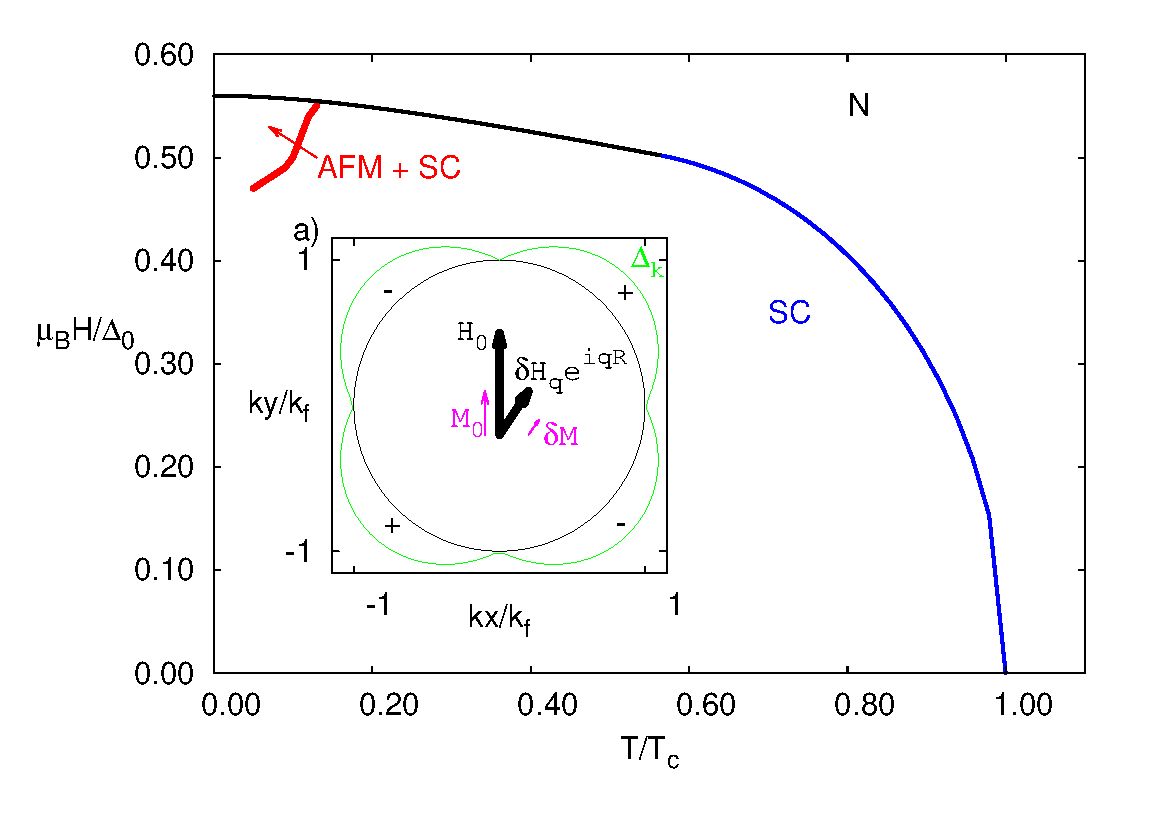
\includegraphics[scale = 0.4]{Fig1.eps}
\caption{ 
	\label{fig:model}
	(Color online)
	An outline of the coexistence phase in the high field low temperature region of a Pauli limited material with $d$-wave symmetry.
	a) We consider two-dimensional Pauli-limited $d$-wave superconductor with circular Fermi surface (FS). 
	The order parameter is $\Delta_\vk = \Delta_0 (T,H) \sin 2\theta_\vk $; 
	the magnetic field has large uniform component $\vH_0$ and spatially varying perturbation $\delta \vH_\vq$
	with wave vector $\vq$. 
}
\end{figure}
%%%%%%%%%%%%%%%%%%%%%%%%%%%%%%%%%%%%%%%%%%%%%%%%%%%%%%%%%%%%%%%%%%%%%%%%%%%%%%%%%


%~~~~~~~~~~~~~~~~~~~~~~~~~~~~~~~~~~~~~
%\emph{Model.}
%~~~~~~~~~~~~~~~~~~~~~~~~~~~~~~~~~~~~~
%
To investigate the interplay of superconductivity and magnetic order in external field,  
we consider a mean-field SC Hamiltonian of 2D electrons with cylindrical FS,
interacting with uniform magnetic field $\vH_0$ through Zeeman term: 
$
\cH = \cH_{0} + V  
$
\bea
\label{eq:modelH} 
\cH_{0} = \sum_{\vk \mu} \xi_\vk c^\dag_{\vk \mu} c_{\vk,\mu} 
+ \sum_\vk \left( \Delta_\vk c_{\vk,\uparrow}^\dag c_{-\vk,\downarrow}^\dag + h.c. \right) 
\\
+ \mu_\sm{B} \sum_{\vk \mu \nu} c^\dag_{\vk\mu} \, \vsigma_{\mu\nu} \vH_0 \, c_{\vk\nu}  
\nonumber  
\eea
and for linear response we include a $\vq$-dependent perturbation 
of the magnetic field $\delta\vH(\vR) = \delta\vH_\vq e^{i\vq\cdot\vR}$, 
$V = \mu_\sm{B} \sum_{\vk \mu \nu} c^\dag_{\vk+\vq \mu}  \, \vsigma_{\mu\nu} \delta\vH_\vq \, c_{\vk \nu}  $, where $\mu_\sm{B}$ is the magnetic moment of electron.
The electronic dispersion in the normal state is $\xi_{\vk}=\frac{\vk^2}{2m^*}-\epsilon_F$.  
The resulting magnetization has uniform part and $\vq$-dependent perturbation:
\be
M_\alpha(\vR) = M_{0\alpha}(\vH_0) + %\delta M_\alpha(\vR)
%\\
%\delta M_\alpha(\vR) = 
\chi_{\alpha\beta} (\vq) \delta H_\beta e^{i\vq \cdot \vR}
\ee
with 
$\vM_0(\vr,t) = \mu_\sm{B} \langle \vS(\vr,t) \rangle_0 $, 
and susceptibility~\cite{mahan}: 
\bea
%&& \vM_0(\vr,t) = \mu_\sm{B} \langle \vS(\vr,t) \rangle_0 \,,
%\\
&& \chi_{\alpha\beta}(\vr, t)= \frac{i \mu_\sm{B}^2}{\hbar} 
\langle [ S_\alpha(\vr,t), S_\beta(0,0) ] \theta(t) \rangle_0 
\\
&& \chi_{\alpha\beta}(\vq)=  
\int d^3 r e^{-i\vq\vr} \int\limits_{0}^{+\infty} dt \, e^{-0^+ t} \,  
\chi(\vr, t)
\label{eq:susdef}
\eea
where 
$\vS(\vr,t) = \sum_{\mu \nu} \psi^\dag_\mu(\vr,t) \, \vsigma_{\mu\nu} \, \psi_{\nu}(\vr,t)$,  
$\psi_{\nu}(\vr,t) = \sum_\vk c_{\vk \nu} (t) \varphi_\nu(\vr)$, 
$c_{\vk \nu} (t) = e^{i\cH_0 t} c_{\vk \mu} e ^{-i \cH_0 t}$; 
subscript $0$ indicates the average over ensemble (\ref{eq:modelH}). 

The temperature and magnetic field dependence of the uniform magnetization $\vM_0$
is known, eg.\cite{Vorontsov06_FLfflo}
and here we discuss the susceptibility $\chi_{\alpha\beta}(\vq)$, since 
it determines the magnetic instability into 
an SDW state, 
and the RKKY-type interaction between localized moments. 
To calculate the susceptibility (\ref{eq:susdef}) in superconducting state, we diagonalize 
the Hamiltonian (\ref{eq:modelH}) by the 
Bogoliubov transformation, 
$c_{\vk \mu} = u_\vk \gamma_{\vk \mu} + (i\sigma_2)_{\mu\nu} v_\vk^* \gamma^\dag_{-\vk \nu} $
%
\be 
\cH_0 = \sum_{\vk \mu} \epsilon_{\vk \mu} \gamma^\dag_{\vk \mu} \gamma_{\vk \mu} \,,
\quad
\epsilon_{\vk\mu} =\sqrt{ \xi_{\vk}^2 + \Delta_{\vk}^2 }  \pm \mu_\sm{B} H_0 
\ee 
with spin-independent coefficients, 
$\epsilon_\vk = \sqrt{ \xi_{\vk}^2 + \Delta_{\vk}^2 }$, 
\be
u_{\vk}= \sqrt{\frac{1}{2}\left( 1+\frac{\xi_{\vk}}{\epsilon_\vk}  \right)} \,, \quad 
v_{\vk}= \sgn(\Delta_\vk) \sqrt{\frac{1}{2}\left( 1-\frac{\xi_{\vk}}{\epsilon_\vk} \right)}
\ee
%u_{\vk}=\sqrt{\frac{1}{2}\left( 1+\frac{\xi_{\vk}}{\sqrt{\Delta_{\vk}^2+\xi_{\vk}^2}} \right)} \\
%v_{\vk}= \sgn(\Delta_\vk) \sqrt{\frac{1}{2}\left( 1-\frac{\xi_{\vk}}{\sqrt{\Delta_{\vk}^2+\xi_{\vk}^2}} \right)}

In the presence of external magnetic field $\vH_0$ the spin-rotational symmetry is broken, 
and one introduces 
%longitudinal and transverse 
%two inequivalent direction of the wave-vector dependent magnetization: 
(a) $\delta \vM(\vq) \parallel \vH_0$ (longitudinal response), and 
(b) $\delta \vM(\vq) \perp \vH_0$ (transverse response). 
The general expressions for the two components of the susceptibility are: 
%%%%%%%
\begin{widetext}
\bea
\label{eq:chi}
\chi_{\parallel}( \vq ) = -\mu_\sm{B}^2 \sum\limits_{\vk\mu}  \left\{
\frac{ [ f(\epsilon_{\vk_-\mu}) -f(\epsilon_{\vk_+\mu}) ] ( u_{\vk_+}u_{\vk_-}+v_{\vk_+}v_{\vk_-} )^2} 
     { \epsilon_{\vk_-\mu}-\epsilon_{\vk_+\mu} } 
-\frac{ [ 1-f(\epsilon_{\vk_-\mu})-f(\epsilon_{\vk_+\opp{\mu}}) ] ( u_{\vk_+}v_{\vk_-}-v_{\vk_+}u_{\vk_-} )^2 }
	{ \epsilon_{\vk_-\mu}+\epsilon_{\vk_+\opp{\mu}} }
\right\}
\\
\chi_{\perp}( \vq ) = -\mu_\sm{B}^2 \sum\limits_{\vk\mu} \left\{
\frac{ [ f(\epsilon_{\vk_-\mu})-f(\epsilon_{\vk_+\opp{\mu}}) ] ( u_{\vk_+}u_{\vk_-}+v_{\vk_+}v_{\vk_-} )^2 }
	{ \epsilon_{\vk_-\mu}-\epsilon_{\vk_+\opp{\mu}} } 
-\frac{ [ 1-f(\epsilon_{\vk_- \mu})-f(\epsilon_{\vk_+\mu}) ] ( u_{\vk_+}v_{\vk_-}-v_{\vk_+}u_{\vk_-} )^2 }
	{\epsilon_{\vk_-\mu}+\epsilon_{\vk_+\mu}} 
	\right\}
	\nonumber
\eea
\end{widetext}
%%%%%%%
where 
$f(\epsilon) = [ \exp(\epsilon/T)+1 ]^{-1}$ is the Fermi distribution, 
and momenta are shifted by the magnetization wave vector $\vk_\pm = \vk \pm \vq/2$. 
Notation $\opp{\mu}$ means spin state opposite to $\mu = \pm1$. 

%~~~~~~~~~~~~~~~~~~~~~~~~~~~~~~~~~~~~~
%\emph{Results.}
%~~~~~~~~~~~~~~~~~~~~~~~~~~~~~~~~~~~~~
%
In the normal state, by setting $\Delta_\vk = 0$ in the general expression above, one obtains the familiar 
Lindhard function,  
\bea
\label{eq:chiN}
\chi^N_{\parallel}(q) =- \mu_\sm{B}^2\sum\limits_{\vk\mu} 
	\frac{ f(\xi_{\vk\mu})-f(\xi_{\vk+\vq \mu})}
	{ \xi_{\vk \mu}-\xi_{\vk+\vq \mu} } 
	\\
\chi^N_{\perp}(q) =- \mu_\sm{B}^2 \sum\limits_{\vk \mu} 
	\frac{ f(\xi_{\vk\mu})-f(\xi_{\vk+\vq \opp{\mu}}) }
	{ \xi_{\vk \mu}-\xi_{ \vk+\vq \opp{\mu}} }  \nonumber
\eea
where $\xi_{\vk \mu} = \frac{k^2}{2m^*}-\epsilon_F \pm \mu_\sm{B} H_0$ are electron excitation 
energies in magnetic field. 
At zero temperature the Fermi functions are step-functions, 
and the integration over momenta can be done analytically; 
in two dimensions we get 

\begin{widetext}
\bea
\frac{\chi^N_\parallel(q)}{\chi_0} = 
1-\frac12 \theta(q-2 k_{f\uparrow})   \sqrt{1-\left( \frac{2 k_{f\uparrow}}{q} \right)^2 } 
 -\frac12 \theta(q-2 k_{f\downarrow}) \sqrt{1-\left( \frac{2 k_{f\downarrow}}{q} \right)^2 }
   \\
\frac{\chi^N_\perp(q)}{\chi_0} = 1-\frac12 \theta(q-k_{f\uparrow}-k_{f\downarrow}) \left[
 \sqrt{ \left( 1 + \frac{ k_{f\uparrow}^2 - k_{f\downarrow}^2}{q^2} \right)^2  - \left( \frac{2k_{f\uparrow}}{q} \right)^2 } 
+\sqrt{ \left( 1 + \frac{ k_{f\downarrow}^2 - k_{f\uparrow}^2}{q^2} \right)^2  - \left( \frac{2k_{f\downarrow}}{q} \right)^2 } 
\right]
\eea
\end{widetext}
Here $\chi_0 = 2 \mu_\sm{B}^2 N_F$ is Pauli susceptibility at $q=0$, 
and $k_{f\uparrow\downarrow} ^2 = k_f^2 ( 1 \mp \mu_\sm{B} H_0/\epsilon_F)$ 
are the Fermi momenta for two spin projections. 
One notices that the parallel component shows two kinks, at $q=2k_{f\uparrow}$ and $2k_{f\downarrow}$, 
when the Fermi surfaces of up- and down-spins touch at a single point, whereas transverse component involves 
opposite spins which results in only one critical 
$q=k_{f\uparrow} + k_{f\downarrow}$. 
Generally, the value and behavior of $\chi(q)$ is determined by the properties of the dispersion 
$\xi_\vk$ at hot spots, where $\xi_{\vk+\vq} = -\xi_\vk$. Near those spots both denominator and numerator 
in $\chi$ are close to zero, and the value of the susceptibility is determined by the phase space, 
which is a function of $\vk$-space dimensionality and the shape of the Fermi surface. For example, 
in one dimensional case or for Fermi surfaces with flat parts the susceptibility is logarithmically divergent. 
\cite{roshen83_spin_sus}

%~~~~~~~~~~~~~~~~~~~~~~~~~~~~~~~~~~~~~
%\section{Superconducting State}
%~~~~~~~~~~~~~~~~~~~~~~~~~~~~~~~~~~~~~
%
%%%%%%%%%%%%%%%%%%%%%%%%%%%%%%%%%%%%%%%%%%%%%%%%%%%%%%%%%%%%%%%%%%%%%%%%%%%%%%%%%
\begin{figure}[t]
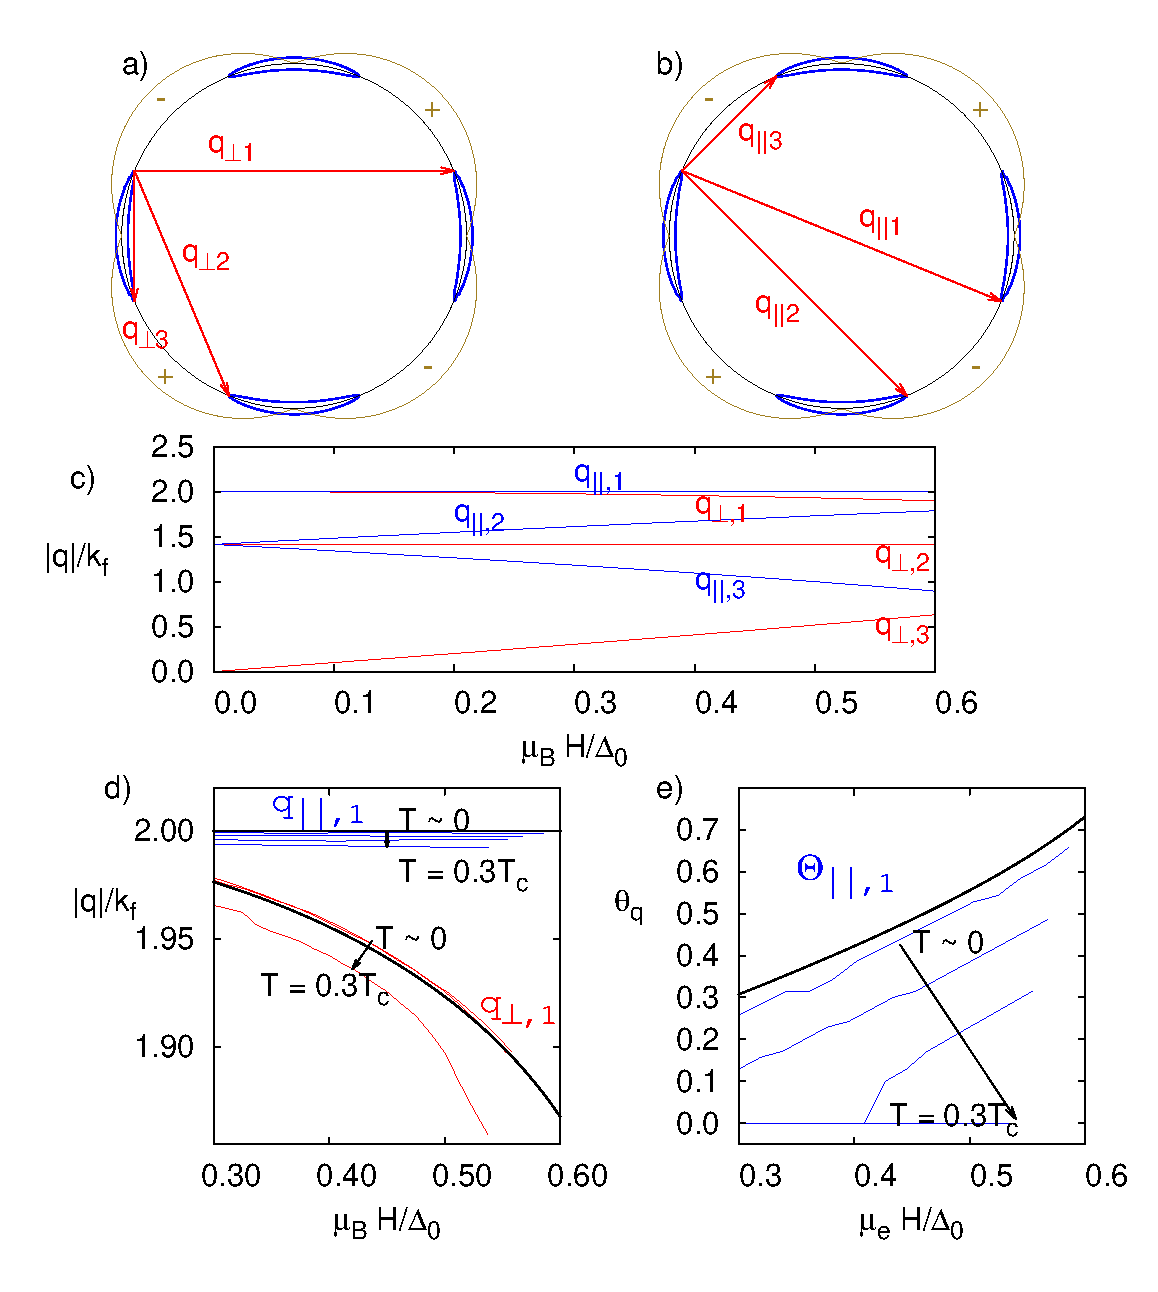
\includegraphics[width=0.95\linewidth]{Fig2.eps}
%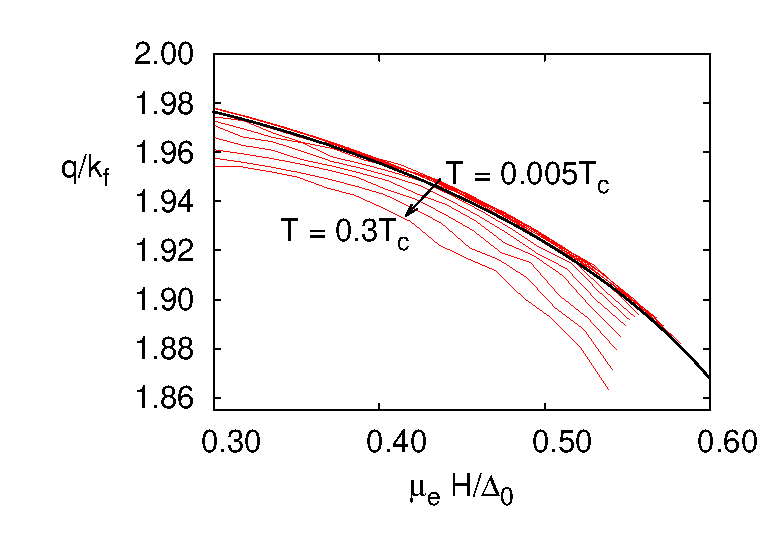
\includegraphics[width=0.75\linewidth]{Fig2d.eps}
%\includegraphics[width=0.95\linewidth]{../sus_enhancement_paper/new_figs/Bananas_with_q_T.eps}
\caption{ 
	\label{fig:qq} 
	(Color online) 
	Magnetic field produces pockets of low energy spin-down excitations near the nodes 
	of the order parameter (blue line regions: a, b). 
	The enhancement of the spin susceptibility in the d-wave superconductor occurs 
	when magnetization vector connects quasiparticle pockets with opposite sign gap 
	for transverse response (a), and same sign gap for longitudinal response (b). 
	(c) the magnitude of the magnetization vectors as a function of the field at zero 
	temperature, determined by geometry (a,b); 
	(d, e) finite temperature deviations (colored) of the optimal magnetization vector from those found from geometry (black) (a,b). 
} 
\end{figure}
%%%%%%%%%%%%%%%%%%%%%%%%%%%%%%%%%%%%%%%%%%%%%%%%%%%%%%%%%%%%%%%%%%%%%%%%%%%%%%%%%

In the unconventional superconducting $d$-wave state we want to find the
maximal values of susceptibility and the corresponding 
magnetization wave vectors. 
The presence of the symmetry-protected nodes in the gap function results in 
spin-down quasiparticles with negative energies. This produces new Fermi surface pockets near the nodes 
of $\Delta_\vk$,\cite{kato11_sc_afm} and partially destroys superconductivity (Pauli pair-breaking). 
The longitudinal $\vq \to 0$ limit gives the diamagnetic response, which in unconventional superconductors 
is modified due to the nodal quasiparticles, $\chi(0)/\chi_0 \sim \mu_\sm{B} H_0/\Delta_0$. The opposite spin pairing nature of the 
transverse response however, ensures $\chi_\perp (0) = 0$.  
 
The analytic analysis of Eqs.~(\ref{eq:chi}) in general is quite difficult, 
and the result will strongly depend 
on the topology of the Fermi surface, field and temperature. 
However, the important factors to find the vectors $\vq$ that maximize the susceptibility 
can be stated for $T=0$ limit. 
These vectors are shown in Fig.~\ref{fig:qq}(a),(b) for $\chi_\perp$ and $\chi_\parallel$,  
and they connect the sharp ends of the spin-down quasiparticle pockets, given by 
$\epsilon_{\vk,\downarrow}=\sqrt{\xi_\vk^2 + \Delta_\vk^2}-\mu_\sm{B} H=0$. 
This result is in accord with the enhanced quasiparticle scattering with those vectors 
observed in \cite{McElroy03_qp_BSCCO}. 
In the vicinity of such common point, 
$\epsilon_{\vk_+,\downarrow} \approx \epsilon_{\vk_-,\downarrow} \approx 0$ and the 
denominators of first term in longitudinal $\chi_\parallel$ 
and second term in transverse $\chi_\perp$ response, can be 
expanded as $\vv_+ \delta\vk + \vv_-\delta\vk$, in regions allowed by the distribution 
functions in numerators. The contribution to $\chi$ is greatest when denominator is smallest, 
when the group velocities $\vv_\pm = \grad_\vk \epsilon_{\vk_\pm,\downarrow}$ are the 
smallest, \ie near the sharp ends of the banana-like regions, where quasiparticle 
velocity is related to the opening rate of the gap 
$v_\Delta = \partial \sqrt{v_F^2k_\perp^2 + \Delta_0^2 \sin^2 2\phi} / \partial (k_F \phi)
\sim v_F (\Delta_0/\epsilon_F) \ll v_F$. 
The actual magnitude of $\chi$ is determined by the available phase space given by 
complicated FS overlap in 2D $\vk$-plane, 
and the superconducting coherence factors.  
The longitudinal first term is maximized when 
the magnetization vector $\vq$ connects the same $\Delta_\vk$-sign 
pockets, making 
$ ( u_{\vk_+}u_{\vk_-}+v_{\vk_+}v_{\vk_-} ) $ 
the most positive and largest with $v_{\vk_+}v_{\vk_-}>0$; 
similarly, largest $\chi_\perp$ is reached when $ ( u_{\vk_+}v_{\vk_-}-v_{\vk_+}u_{\vk_-} ) $
is most positive. This occurs at vectors, connecting quasiparticle pockets with the 
opposite sign of $\Delta_{\vk_\pm}$. 
The $T=0$ length of the magnetization vectors as function of magnetic field 
is shown in Fig.~\ref{fig:qq}(c).

We confirm this analysis numerically, 
since the size of the new FS pockets is small, having energy scale of 
$\mu_\sm{B}H_0 \sim \Delta_0 \ll \epsilon_F$ 
and momentum space scale $1/\xi_0 \ll k_F$. This means that the changes with temperature 
and field to $\vq$s and to $\chi$ can be considerable, and difficult to treat 
analytically. 
As an example, in Fig.~\ref{fig:qq}(d,e) 
we show the $T$-induced deviations of optimal $\vq$ vectors from their $T=0$ values, 
found by numerically finding the maximum of the susceptibility $\chi(\vq)$, 
and corresponding $\vq$, at given $T$ and $H_0$. 
We note that at finite $T$ the magnetization vector is smaller than zero-$T$ one in 
transverse components, and results in smaller overlap of the Fermi pockets.
On the other hand for longitudinal component the overlap is increasing with temperature. 

The nodal ordering vector  $\vq_{\perp 3}$ is the most likely candidate 
from experimental point of view $[0.44,0.44]\pi/a$ \cite{Kenzelmann10_Qphase} and it also agrees with 
the size of the $\alpha$-FS pocket of \cecoin, \cite{suzuki11_sdw_vortex}
and the choice of the microscopic parameters, 
$\Delta_0/\epsilon_F \sim 0.6 meV/0.5 eV \sim 0.001$ \cite{Allan2013_stm115,Maehira03_fs115}. 
The reduction of  $\vq_{\perp 1}$ with temperature is small, 
and is of the order of one percent over $0.3 T_c$-range. Similar size reduction of 
ordering vector was observed in \cite{Kenzelmann10_Qphase} when temperature 
was changed from 60 mK ($0.025 T_c$) to 150 mK ($0.06 T_c$). 
$\vq_{\perp 3}$ also follows the observed \cite{Kenzelmann10_Qphase} slight upward variation with field. 

 %%%%%%%%%%%%%%%%%%%%%%%%%%%%%%%%%%%%%%%%%%%%%%%%%%%%%%%%%%%%%%%%%%%%%%%%%%%%%%%%%
\begin{figure}[t]
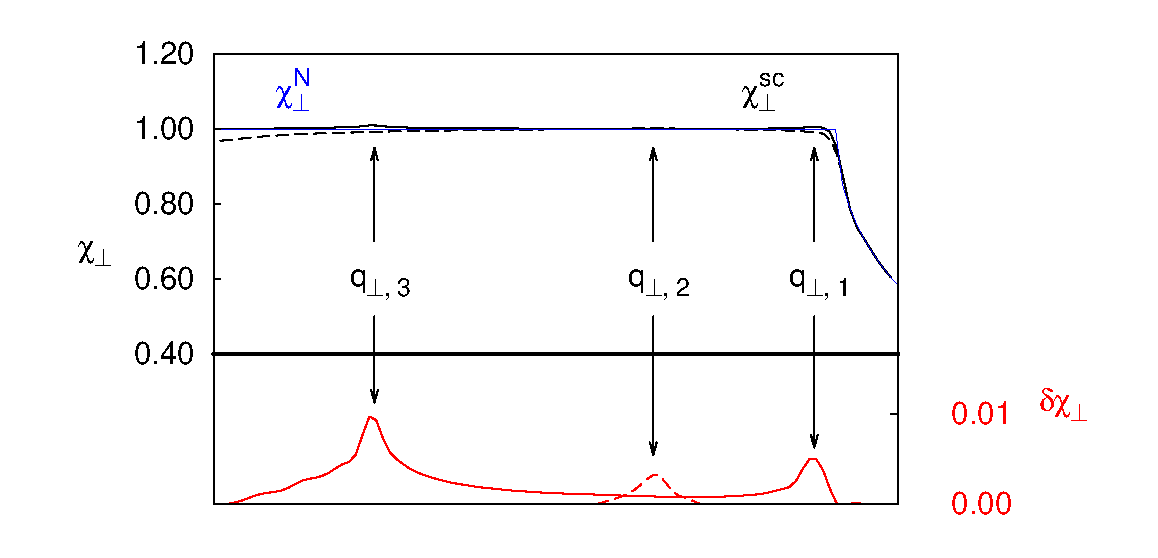
\includegraphics[width=0.95\linewidth]{Fig3.eps}
\caption{
	\label{fig:chi_enh}
	(Color online)
	The $T=0$ normalized susceptibility in the superconducting (black) and normal states (blue) as a function of $q$. 
We set $\mu_\sm{B} H = 0.5\Delta_0$, close to Pauli limiting field $\mu_\sm{B} H_\sm{P}/\Delta_0 = 0.56$, 
and $\Delta_0/\epsilon_F = 0.005$. Transverse susceptibility shows enhancement over the normal state $\chi^N(q)$ 
for three wave vectors, two values of $q$ for nodal-$\vq$ orientation $\vq_{\perp 1,3}$ (solid), 
and one value for $\vq || \vq_{\perp 2}$ (dashed), 
in accordance with Fig.~\ref{fig:qq}(a,c). 
The lower pane shows $\delta\chi_\perp(q) = \chi_\perp^{sc}(q) - \chi_\perp^{N}(q)$. 
%
%(b) Same for longitudinal component. 
%Solid red for directions along anti-nodal direction $\vq_{\parallel 2} || \vq_{\parallel 3}$, 
%and dashed for $\vq_{\parallel 1}$.  
%
The maximal enhancement $\delta \chi_{\perp}(q)$ occurs at wave vectors 
$\vq_{\perp 3}$ and is of the 
order $\delta \chi_\perp/\chi_0 \sim \Delta_0/\epsilon_F$. 
}
 \end{figure}
%%%%%%%%%%%%%%%%%%%%%%%%%%%%%%%%%%%%%%%%%%%%%%%%%%%%%%%%%%%%%%%%%%%%%%%%%%%%%%%%%
  

In Fig.~\ref{fig:chi_enh} we plot the transverse susceptibility as a function of magnetic wave vector 
in superconducting state at zero temperature and in 
magnetic field $\mu_\sm{B} H = 0.5\Delta_0$. 
The directions of the $\vq$s are chosen in accordance with Fig.~\ref{fig:qq}.
In this parameter regime, the maximal enhancement of $\chi$ corresponds to the shortest $\vq$.


%For the transverse component it is just below the normal state kink $k_{f\uparrow}+k_{f\downarrow}$, 
%and maximal $\chi^{sc}_\perp(q)$ sits well above the maximal normal state value of $\chi_0$. 
%For the longitudinal component the most enhanced peak is at nearly $2k_f$ - right between the two 
%normal state kinks at $2k_{f\uparrow\downarrow} = 2k_f \sqrt{1\mp \mu_\sm{B}H_0/\epsilon_F}$, 
%and although large, still does not go appreciably above the $\chi_0$ value of the 
%normal state due to the quick drop off the background normal state $\chi$. 


%%%%%%%%%%%%%%%%%%%%%%%%%%%%%%%%%%%%%%%%%%%%%%%%%%%%%%%%%%%%%%%%%%%%%%%%%%%%%%%%%
\begin{figure}[t]
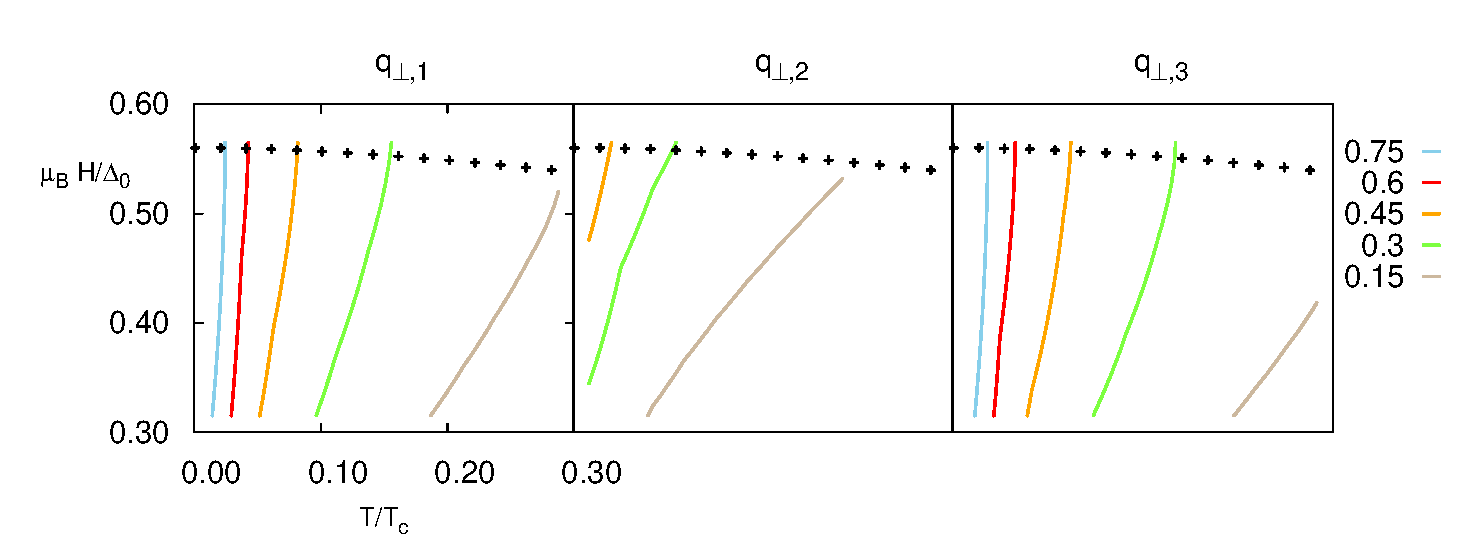
\includegraphics[width=\linewidth]{Fig4.eps}
\caption{ 
	\label{fig:ph.d} 
	(Color online) 
	Contour lines of maximal enhancement of transverse susceptibility $\chi_\perp$ in the $T$-$H$ 
	phase diagram. Different contours correspond to relative enhancements 
	$\delta\chi(q)/\chi_0$ given in percents. 
	The three panels correspond to $\vq$-vectors at those shown in figure \ref{fig:qq}(a). 
	The black bold dotted line is the first order phase transition
	for a Pauli limited $d$-wave superconductor. $\Delta_0 = 0.005\epsilon_F$.
}
\end{figure}
%%%%%%%%%%%%%%%%%%%%%%%%%%%%%%%%%%%%%%%%%%%%%%%%%%%%%%%%%%%%%%%%%%%%%%%%%%%%%%%%%
 
%~~~~~~~~~~~~~~~~~~~~~~~~~~~~~~~~~~~~~
%\emph{Conclusions.}
%~~~~~~~~~~~~~~~~~~~~~~~~~~~~~~~~~~~~~
%
Finally, we present $T$-$H$ phase diagram of a $d$-wave superconductor with Pauli pairbreaking, 
and plot the the contours of maximal susceptibility enhancement in Fig.~\ref{fig:ph.d}. 
We find the self-consistent value of the 
gap amplitude $\Delta_\vk = \Delta(T,H) \sin2\theta_\vk$, (Note $\Delta_0 = \Delta(0,0)$) 
at each $T$ and $H_0$, and then substitute it into Eq.~(\ref{eq:chi}). 
Then we scan over magnetization vectors close to suggested $\vq_i$ to find the maximal value of 
$\chi(\vq)$. In this way we find the optimal wave vector and corresponding maximal $\chi$ for 
given $T$,$H$. 

The magnitude of the $\delta \chi$ becomes positive in the 
upper left corner (low $T$, high $H$). It grows further as we increase field or  
lower temperature. The size of the enhancement over the normal state is 
$\delta\chi/\chi_0 \sim \Delta_0/\epsilon_F$ which is a fraction of a percent in \cecoin. 
Such small enhancement is consistent with the strong magnetic fluctuations in the normal 
state $J(\vq) \chi_0 \approx 1^-$, that become critical only in the presence of SC condensate, where 
$\chi^{RPA}_{\alpha\beta}(\vq)={\chi_{\alpha\beta} (\vq) }/{[1-J(\vq) \chi_{\alpha\beta}(\vq)]}$
diverges. 
The curves of constant 
$\delta\chi(T,H)$ will determine the boundary of the magnetic SDW 
state inside the superconducting phase. 
The slope and the direction of $\delta\chi$ increase in the $T$-$H$ phase diagram is consistent with 
the location of the Q-phase transition in \cecoin, and agrees with the conclusions of 
\cite{kato11_sc_afm}. 

We find that both transverse and longitudinal component can be enhanced over the normal state, 
$\chi_{\perp}(\vq,H_0) > \chi^N_\perp(\vq,\vH_0)$
and
$\chi_{\parallel}(\vq,H_0) > \chi^N_\parallel(\vq,\vH_0)$, but the emergence of a
 longitudinal response is unlikely, because $\delta \chi$ is near numerical accuracy and $\chi_{\parallel}$
 never goes appreciably above $\chi_0$.


In conclusion, we investigated the behavior of spin susceptibility in Pauli-limited 
unconventional superconductors. We found that the field-induced nodal quasiparticles, and the sign-changing 
nature of the gap, leads to the enhancement of the transverse susceptibility component 
inside the superconducting phase. 
As a result, similar enhancement in conventional superconductors, even with strongly anisotropic and even nodal 
gap function, is unlikely. \cite{Machida1981_sdw_sc}
The enhancement is of the order $\delta\chi/\chi_0 \sim \Delta_0/\epsilon_F$ 
and is a strong function of temperature and magnetic field; 
it may result in SDW order formed inside the superconducting phase at low temperatures and 
high fields, consistent with observations in \cecoin.  
There are several magnetization vectors that connect field-induced Fermi pockets, and the 
ordering vector will be determined by the propertis of the 
magnetic interaction $J(\vq)$. 
Enhancement of the longitudinal component is also significant but it occures on the 
background of fast-decreasing normal state $\chi_\parallel^N(\vq)$ and does not lead to 
significant increase over $\chi_0$, unless the magnetic interaction $J(\vq)$ is strongly 
peaked at the same wavevector. 

This research was done with NSF support through grant DMR-0954342. 
ABV acknowledges hospitality of Aspen Center for Physics, and discussions with 
I.~Vekhter. 
 %~~~~~~~~~~~~~~~~~~~~~~~~~~~~~~~~~~~~~~~~~~~~~~~~~~~~~~~~~~~~~~~~~~~~~~~~~~~~~~~
  %~~~~~~~~~~~~~~~~~~~~~~~~~~~~~~~~~~~~~~~~~~~~~~~~~~~~~~~~~~~~~~~~~~~~~~~~~~~~~~~
   %~~~~~~~~~~~~~~~~~~~~~~~~~~~~~~~~~~~~~~~~~~~~~~~~~~~~~~~~~~~~~~~~~~~~~~~~~~~~~~~
    %~~~~~~~~~~~~~~~~~~~~~~~~~~~~~~~~~~~~~~~~~~~~~~~~~~~~~~~~~~~~~~~~~~~~~~~~~~~~~~~
     %~~~~~~~~~~~~~~~~~~~~~~~~~~~~~~~~~~~~~~~~~~~~~~~~~~~~~~~~~~~~~~~~~~~~~~~~~~~~~~~
      %~~~~~~~~~~~~~~~~~~~~~~~~~~~~~~~~~~~~~~~~~~~~~~~~~~~~~~~~~~~~~~~~~~~~~~~~~~~~~~~

\bibliography{mybib}

%~~~~~~~~~~~~~~~~~~~~~~~~~~~~~~~~~~~~~~~~~~~~~~~~~~~~~~~~~~~~~~~~~~~~~~~~~~~~~~~%
\end{document}
%~~~~~~~~~~~~~~~~~~~~~~~~~~~~~~~~~~~~~~~~~~~~~~~~~~~~~~~~~~~~~~~~~~~~~~~~~~~~~~~%
